\documentclass{article}

% Please use the following line and do not change the style file.
\usepackage{icml2021_author_response}

% Recommended, but optional, packages for figures and better typesetting:
\usepackage{microtype}
\usepackage{graphicx}
\usepackage{subfigure}
\usepackage{hyperref}       % hyperlinks
\usepackage{booktabs} % for professional tables
\usepackage{amsfonts}       % blackboard math symbols
\usepackage{nicefrac}       % compact symbols for 1/2, etc.

\usepackage{lipsum}

\begin{document}
% Uncomment the following line if you prefer a single-column format
% \onecolumn

First of all we would like to sincerely thank all reviewers for their very detailed and precise remarks on our work. These comments are very useful to improve many aspects of the article, both on theoretical and numerical points.
\begin{figure}[H]
\vskip -0.1in
\begin{center}
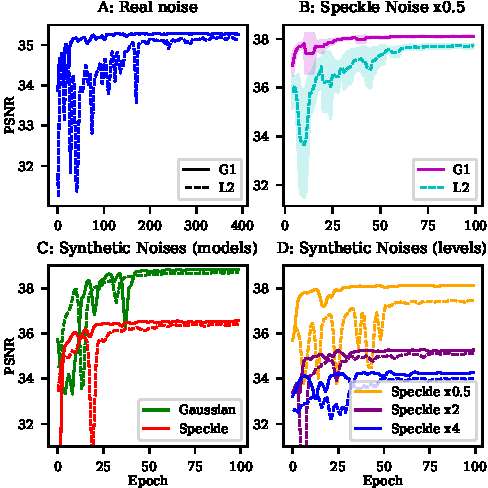
\includegraphics[width=\columnwidth]{fig_review.pdf}
\vskip -0.15in
\caption{PSNR at each epoch on the test set for N-net (G1) or D-net only (L2). A: training on real noise; final performance gain of G1 over L2 is $+0.11dB$. C, D: training on different models/levels of synthetic noise added to ground truth image. C: \textit{Gaussian} and \textit{Speckle} correspond to noises presented in 5.1, that have no and high signal dependency respectively. D: \textit{Speckle} with variance multiplied by 0.5, 2 and 4. B: Mean and SEM over 5 runs.}
\label{fig:review}
\end{center}
\vskip -0.25in
\end{figure}
\paragraph{Contribution of N-net}
We agree that in its original version the several contributions presented in the paper are not properly distinguished.
In the revised manuscript, we propose to highlight the contribution of the N-net to the performance first by adding Fig.~\ref{fig:review}, that show the impact of the N-net on real and several levels of synthetic noise by comparing our model to the D-Net trained with L2 loss (as in N2V, N2S) with every other aspect fixed.
It shows that N-net always improves performances, although not always significantly (this was verified for the 6 datasets considered in the article). Moreover, the addition of the N-net greatly stabilizes the training (see Fig.~\ref{fig:review}B) and improves convergence speed, which enables easier hyperparameters and architecture optimization.
The N-net alone can thus be seen as a modular and \textit{plug-and-play} addition to existing blind denoising models, which always improves performances and convergence.

% explanations:
From the perspective of our framework, the L2 loss can be understood as a particular case of the N-net predicting a constant unit gaussian noise. When the actual noise is significantly different from it (e.g. \textit{Speckle}), the N-net has a stronger impact (see Fig.~\ref{fig:review}C).
From a statistical perspective,  it is known that considering a sufficiently rich noise model is crucial in deconvolution problem for signal estimation (misspecifying the noise density can lead to very poor deconvolution estimators for instance). This was a motivation to introduce the N-net.

Moreover the noise model was shown in the paper to capture several statistical behaviors, which is interesting \textit{per-se} and could allow to further improve performances by predicting signal distribution as in (Laine et al. 2019) and PN2V.

\paragraph{Theory}
R2 concerns about the description of loss function indicate that we did not provide enough details to support the proposed loss. It is obtained as an approximation of the negative loglikelihood of the model which will be stated clearly in the revised version as follows.
%The D-net $\mu_\theta(\Omega_y,g(\Omega_y))$ is indeed thought as a model for the expected value of the signal X given the surrounding receptive field excluding the central pixel. This quantity as an estimate of the signal value would indeed minimize the mean squared error to the ground truth and this is what supervised training with MSE does.
The conditional loglikelihood of the observations is written $ \log p(Y|\Omega_Y) = \log \int p(x,Y|\Omega_Y) \mathrm{d}x = \log \int p(x|\Omega_Y)p(Y|\Omega_Y,x) \mathrm{d}x$ (*), where $p(Y|\Omega_Y,x)$ is given by our observation model, see Eq. (1).
As it is very challenging to obtain samples from the distribution $p(x|\Omega_Y)$ we propose indeed to estimate this integral by $\log p(Y|\Omega_Y,\hat {X})$ where $\hat {X}$ is an estimate of $\mathbb{E}[X|\Omega_Y]$. Our loss function is then supported by the intuition that $\mu_\theta(\Omega_Y,g(\Omega_Y))$ is a good approximation of $\mathbb{E}[X|\Omega_Y]$. Providing theoretical guarantees that this approximation is good remains an open problem as stated in the original paper. Even though this seems similar to N2V and N2S in terms of loss function we would like to stress that writing explicitly (*) provides a different perspective which we believe:
(1) defines a framework to justify theoretically the proposed approximation (challenging issue); (2) highlights the contribution of $\mu_\theta$ and of the noise model.

\paragraph{Other remarks}
As suggested by R1 and R2, we compared our method to the supervised approach. We chose datasets W2S-1,2 \& 3 where the evaluation dataset is distinct from the training dataset and will include this baseline in the revised manuscript.
We found that our method outperforms the supervised approach of $0.11dB$, $0.22dB$ and $0.26dB$ respectively.
This is not in contradiction with the fact that the central pixel is masked at train time: indeed, our method uses beneficially the central pixel at inference.

% can be removed if necessary
Regarding Noise correlation (R4): only 2 of the 6 datasets display correlation in noise, amplified by the network when not taken into account.
Following (Broaddus et al. 2020) we adapted our masking scheme in that case (see 4.3).

We thank R2 for pointing out erroneous analysis of (Krull et al. 2019). Regarding (Prakash et al. 2020a), it seems that joint learning of noise model was introduced in the pre-print version of March 1st, so after we submitted the manuscript. We will update the manuscript accordingly.

Finally, we emphasize that our method is stable, generic (to types of noises), reproducible (fast and easy code available), so we believe it is a powerful tool for experimenters and a good stepping stone for future research.

% [To be removed si besoin de place] Additionally they model the noise variance as an affine function of the signal intensity. We show that the noise variance may follow a more intricate dependency to the signal intensity and design a more general way to model it



Reviewer #2 4/3/2021, 10:03:14 AM
Topic: Use of the central pixel and performance of supervised learning.
In your feedback, you write :
"
We found that our method out-performs the supervised approach of0.11dB,0.22dBand0.26dBrespectively.
This is not in contradiction with the fact that the central pixel is masked at train time: indeed,our method uses beneficially the central pixel at inference.
"
I unfortunately cannot follow this argument. How can the system learn to make use of the central pixel when it is masked during training?

I have two questions regarding this:
1. Could you please explain how the "method uses beneficially the central pixel at inference", when it is not allowed to see it during training?
and
2. Let's assume that it somehow can make some use of the central pixel, how can it surpass (!) the performance of the supervised approach, which is trained to make optimal use of the full receptive field including the central pixel?
I am looking forward to your answers.

Author 4/5/2021, 7:26:38 PM
Topic: Use of the central pixel and performance of supervised learning.
Thank you for your questions.

1. Classical architectures with successive convolutions (such as U-net) impose a dependency upon the central pixel. This is the reason why specific architectures were developed like the directional convolutions (Laine et al. 2019) or strided convolutions (Noise2Kernel - Lee, Jeong 2020). In approaches such as Noise2Void and Noise2Self the dependency upon the central pixel at test time can be tested empirically.

The beneficial use of the central pixel at inference was also observed in Noise2Self (Batson and Royer 2019), described in appendix 5.4: after training with masked pixels, they compare inference with or without masking, and obtain +0.5dB using the central pixel. We obtain comparable gains for all datasets.

Our intuition is that while the information of the masked pixel is redundant with the neighborhood, the convolutional structure of the net probably induces the learning of a dependency upon the central pixel in a useful way. As discussed in paragraph 6, how the central pixel is used during inference remains an open research question.


2. Our architecture and hyperparameters were tuned with the unsupervised setup in mind. We believe that the supervised version of our method that we presented in the rebuttal can still be improved in terms of architecture and optimization, and therefore does not correspond to the upper bound of possible performances.

Also intuitively, perhaps it’s easier to learn a good denoiser with masking because it forces the network to make better use of the neighborhood rather than overfitting on the central pixel. An interesting perspective would be to use the central pixel in a sensible way both at train and test time.

We hope this answers your questions.


\end{document}
